\section{Problem Setup}
\label{sec:preliminaries}

We consider a target architecture consisting of a single software processor and multiple hardware (ASIC/FPGA) components. Software tasks execute sequentially on the CPU, while hardware tasks without dependencies can execute in parallel. Communication between tasks assigned to different platforms incurs an interconnect transfer cost, modeled as an edge-dependent communication delay. Assignments must satisfy a global hardware area constraint. The goal of HW/SW partitioning is to assign tasks to hardware or software to minimize end-to-end execution time under this constraint.

\subsection{Problem formulation}
We are given a task graph $\gG(\gV,\gE)$ with $|\gV|=n$ nodes and $|\gE|=m$ edges, modeled as a directed acyclic graph (DAG), as shown in Figure~\ref{fig:sampletaskgraph}. Each node $i \in \gV$ has software and hardware execution costs $t_i^{sw}$ and $t_i^{hw}$, respectively, and requires hardware area $A_i$ if assigned to hardware. Each edge $(j,i)\in\gE$ represents a precedence dependency from task $j$ to task $i$, with communication cost $C_{ji}$ incurred when the two endpoint tasks are assigned to different platforms.

\begin{figure}[!htbp]
\centering
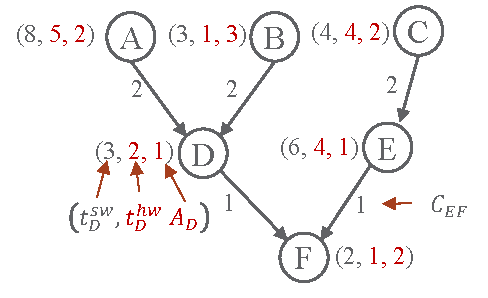
\includegraphics[width=0.5\linewidth]{Figures/introduction/taskgraph.pdf}
\caption{Sample task graph for HW/SW partitioning. Each node shows its software cost, hardware cost, and required hardware area. Directed edges indicate task dependencies, and edge labels represent communication cost when connected tasks are assigned to different types.}
\label{fig:sampletaskgraph}
\end{figure}

We represent a discrete HW/SW partition using a binary vector $\vp \in \{0,1\}^n$, where $p_i=1$ denotes hardware assignment and $p_i=0$ denotes software assignment for node $i$. Since software tasks share a single processor, the final makespan also depends on their execution order. Let $\pi^{sw}$ denote a valid rank-based order over software tasks, where
\begin{equation}
\pi_i^{sw} < \pi_j^{sw}
\;\Longrightarrow\;
i \prec_{\pi^{sw}} j,
\end{equation}
meaning that task $i$ is scheduled before task $j$ on the software processor.
Given an assignment $\vp$ and software order $\pi^{sw}$, let $(\vs, \vf)\gets \mathrm{Sched}(\vp,\pi^{sw})$ denote the induced schedule that returns the corresponding start-time and finish-time vectors $\vs$ and $\vf$. The makespan under assignment $\vp$ and software order $\pi^{sw}$ is defined as
\begin{equation}
M(\vp,\pi^{sw}) = \max_{i\in\gV} f_i.
\label{eq:true_makespan}
\end{equation}

Our goal is to minimize makespan under the hardware area budget:
\begin{align}
\min_{\vp \in \{0,1\}^n,\;\pi^{sw}} \quad
& M(\vp,\pi^{sw}) = \max_{i\in\gV} f_i
\label{eq:true_obj}\\
\text{s.t.}\quad
& (\vs,\vf)=\mathrm{Sched}(\vp,\pi^{sw}),
\label{eq:true_sched}\\
& \sum_{i\in\gV} p_i A_i \le A_{\max},
\label{eq:true_area}\\
& f_i = s_i + \underbrace{p_i t_i^{hw} + (1-p_i)t_i^{sw}}_{\mathrm{Execution}},
\qquad \forall i\in\gV,
\label{eq:true_finish}\\
& s_i \ge f_j + \underbrace{\mathbb{I}[p_j \neq p_i]\, C_{ji}}_{\mathrm{Communication}},
\qquad \forall (j,i)\in\gE,
\label{eq:true_pred}\\
& s_j \ge f_i,
\qquad \forall i,j\in\gV: p_i=p_j=0
\text{ and } i \prec_{\pi^{sw}} j,
\label{eq:true_sw_serial}\\
& s_i \ge 0,
\qquad \forall i\in\gV.
\label{eq:true_nonneg}
\end{align}

Equation~\eqref{eq:true_finish} defines the finish time of each task under the chosen assignment. Equation~\eqref{eq:true_pred} enforces precedence constraints together with inter-platform communication delay. Equation~\eqref{eq:true_sw_serial} enforces sequential execution of software-assigned tasks according to the order $\pi^{sw}$. Hardware-assigned tasks may execute in parallel as long as the precedence constraints are satisfied.


\subsection{Differentiable Relaxation of the Discrete Problem}

Directly optimizing Equations~\eqref{eq:true_obj}--\eqref{eq:true_nonneg} is difficult because both the placement vector $\vp \in \{0,1\}^n$ and the software order $\pi^{sw}$ are discrete. In \diffgnn, we therefore relax the binary assignment vector $\vp$ to a continuous vector $\tilde{\vp}\in[0,1]^n$, where $\tilde{p}_i$ denotes the confidence of assigning task $i$ to hardware. To approximate the discrete software order $\pi^{sw}$, the GNN also predicts a continuous software-priority vector $\tilde{\vpi}^{sw}\in[-1,1]^n$. These values encode relative precedence among software tasks: if $\tilde{\pi}_i^{sw} > \tilde{\pi}_j^{sw}$, then the relaxed model prefers $i \prec j$. Sorting $\tilde{\vpi}^{sw}$ induces a discrete rank-based order that approximates $\pi^{sw}$.

Under this relaxation, the execution-time expression in Equation~\eqref{eq:true_finish} becomes
\begin{equation}
\tilde{t}_i(\tilde{\vp})
=
\tilde{p}_i t_i^{hw} + (1-\tilde{p}_i)t_i^{sw},
\label{eq:soft_exec_i}
\end{equation}
and the communication term in Equation~\eqref{eq:true_pred} is approximated by
\begin{equation}
\tilde{c}_{ji}(\tilde{\vp})
=
|\tilde{p}_j-\tilde{p}_i|\, C_{ji}.
\label{eq:soft_comm_ji}
\end{equation}

Similarly, instead of the discrete schedule $(\vs,\vf)=\mathrm{Sched}(\vp,\pi^{sw})$, we define a differentiable surrogate scheduler
\begin{equation}
(\tilde{\vs},\tilde{\vf})
=
\widetilde{\mathrm{Sched}}(\tilde{\vp},\tilde{\vpi}^{sw}),
\label{eq:soft_sched}
\end{equation}
which approximates the precedence, communication, and software-serialization constraints in Equations~\eqref{eq:true_pred}--\eqref{eq:true_sw_serial}.

The max operator appearing in the makespan and readiness computations is not differentiable. We therefore replace it with the smooth maximum operator
\begin{equation}
\mathrm{SMax}_{\beta}(\{a_k\})
=
\frac{1}{\beta}\log\sum_k e^{\beta a_k},
\label{eq:smax_beta}
\end{equation}
where $\beta>0$ controls the sharpness of the approximation. As $\beta$ increases, $\mathrm{SMax}_{\beta}$ approaches the standard max operator.

\paragraph{\textbf{Precedence relation of Equation~\eqref{eq:true_pred}}}
Let $\Pred(i)$ denote the set of predecessors of node $i$. The relaxed DAG-readiness term is defined as
\begin{equation}
s_i^{dag}
=
\begin{cases}
0, & \Pred(i)=\emptyset,\\[4pt]
\mathrm{SMax}_{\beta}
\Big(
\{\, \tilde{f}_j + \tilde{c}_{ji}(\tilde{\vp}) \mid j \in \Pred(i)\,\}
\Big), & \text{otherwise},
\end{cases}
\label{eq:soft_rdag}
\end{equation}
which approximates the earliest time at which task $i$ becomes ready from the precedence perspective of Equation~\eqref{eq:true_pred}.

\paragraph{\textbf{SW relation of Equation~\eqref{eq:true_sw_serial}}}
To capture serialization on the software processor in Equation~\eqref{eq:true_sw_serial}, we define the relaxed software-readiness term as
\begin{equation}
s_i^{sw}
=
\mathrm{SMax}_{\beta}
\Big(
\{\, \tilde{f}_j + \phi_{sw}(\tilde{\pi}_j^{sw}, \tilde{\pi}_i^{sw}) \mid j \neq i\,\}
\Big),
\label{eq:soft_rsw}
\end{equation}
where $\phi_{sw}(\cdot)$ is a differentiable ordering function that maps the relative priority difference between tasks $j$ and $i$ to a soft serialization penalty. Intuitively, if $\tilde{\pi}_j^{sw}$ indicates that task $j$ should execute before task $i$, then the contribution of $\tilde{f}_j$ to $s_i^{sw}$ becomes stronger. The explicit construction of $\phi_{sw}$ is introduced later in the proposed method.

\paragraph{\textbf{Soft makespan of Equation~\eqref{eq:true_makespan}}}
The relaxed start and finish times are then
\begin{equation}
\tilde{s}_i
=
\mathrm{SMax}_{\beta}\big(\{s_i^{dag},\, s_i^{sw}\}\big),
\label{eq:soft_start}
\end{equation}
\begin{equation}
\tilde{f}_i
=
\tilde{s}_i + \tilde{t}_i(\tilde{\vp}),
\label{eq:soft_finish}
\end{equation}
which mirror the discrete scheduling relations in Equations~\eqref{eq:true_finish}--\eqref{eq:true_sw_serial}.

Let $\Sink(\gG)$ denote the set of sink nodes in $\gG$. The differentiable surrogate makespan is defined as
\begin{equation}
\widetilde{M}(\tilde{\vp},\tilde{\vpi}^{sw})
=
\mathrm{SMax}_{\beta}\big(\{\, \tilde{f}_i \mid i \in \Sink(\gG)\,\}\big).
\label{eq:soft_makespan_symbol}
\end{equation}

\paragraph{\textbf{Area of Equation~\eqref{eq:true_area}}}
To encourage feasibility under the hardware budget in Equation~\eqref{eq:true_area}, we use the differentiable area penalty
\begin{equation}
\mathcal{L}_{\mathrm{area}}(\tilde{\vp})
=
\left[
\max\left(
0,\;
\sum_{i\in\gV}\tilde{p}_i A_i - A_{\max}
\right)
\right]^2.
\label{eq:l_area}
\end{equation}

\paragraph{\textbf{Relaxed objective}}
The relaxed objective optimized by \diffgnn is therefore
\begin{equation}
\mathcal{L}_{\mathrm{relax}}(\tilde{\vp},\tilde{\vpi}^{sw})
=
\widetilde{M}(\tilde{\vp},\tilde{\vpi}^{sw})
+
\lambda_a \mathcal{L}_{\mathrm{area}}(\tilde{\vp}).
\label{eq:relaxed_obj}
\end{equation}

Thus, while the original problem minimizes makespan over the discrete placement vector $\vp$ and software order $\pi^{sw}$, \diffgnn is trained by minimizing the continuous surrogate in Equation~\eqref{eq:relaxed_obj}. Auxiliary execution, communication, and regularization terms used in practice are introduced later in the proposed method.
